\documentclass[urop]{socreport}
\usepackage{fullpage}

\usepackage{url}
\usepackage{amsmath,amsthm,amsfonts}
\usepackage{algorithm,algorithmic}
\usepackage[dvips]{color}
\usepackage{algorithm,algorithmic}
\usepackage{graphicx}
\usepackage{CJKutf8}

\usepackage{tikz}
\usetikzlibrary{trees}
\usetikzlibrary[positioning]
\usetikzlibrary{calc}
\usetikzlibrary{decorations.pathmorphing}
\usetikzlibrary{fit}
\usetikzlibrary{backgrounds}
\tikzstyle{level 1}=[level distance=4cm, sibling distance=3.5cm]
\tikzstyle{level 2}=[level distance=4cm, sibling distance=2cm]
\tikzstyle{bag} = [text width=4em, text centered]
\tikzstyle{end} = [circle, minimum width=3pt,fill, inner sep=0pt]
\tikzstyle{fork} = [circle, minimum width=3pt,fill, inner sep=0pt]

\begin{document}
\pagenumbering{roman}
\title{Word Sense Prediction Using Decision Trees}
\author{Heng Low Wee \\ (U096901R)}
\projyear{2010/11}
\projnumber{U079330}
\advisor{A/P Min-Yen Kan}
\deliverables{
	\item Report: 1 Volume
	\item Source Code: 1 DVD}
\maketitle
\begin{abstract}
\paragraph{}
%%%From Aobo: Better to show the motivation of reducing the size and time, which is to make it more applicable in a real time software like DICE translator.
%%% updated
Word sense disambiguation (WSD) is a key task in Natural Language Processing. There are many existing systems that are able to achieve good performance in \textsc{SensEval} and \textsc{SemEval} tasks. However, few systems discuss about reducing the size of the training model and the time taken for the WSD process. For WSD systems to be applied onto real-time softwares, such as building a WSD software for mobile devices, they need to be scaled down in terms of its training model size, and be responsive to enhance user experience. With that, we propose the idea of building a WSD system that is light-weight and speedy.

\paragraph{}
%%%From Aobo: maybe indicate what is the data size and processing time before reducing, or show how many percentage it has reduced.
%%% updated
In this report, we study how we can adopt using Decision Trees to predict the word senses of ambiguous words. Our system aims to reduce the size of the training model and the time taken to predict word senses. In our implementation, we reduced both the size of our training model and the time taken by over 98\%, with our system performing speedily when disambiguating sentences, while retaining a reasonable performance for accuracy.

\begin{descriptors}
	\item I.2.7 Natural Language Processing
\end{descriptors}
\begin{keywords}
	decision tree,  word sense disambiguation, word sense, ambiguous
\end{keywords}
\begin{implement}
\begin{flushleft}
\hspace{5 mm}Software: Java, Perl, Weka 3.\\
\hspace{5 mm}Hardware: MacBook Pro, Intel Core 2 Duo 2.4GHz, 4GB Memory.
\end{flushleft}
\end{implement}
\end{abstract}

\begin{acknowledgement}
\paragraph{}
First of all, I would like to thank my supervisor, A/P Min-Yen Kan, for his support throughout the entire duration of this project. He was very patient, and always willing to answer my questions whenever I had any doubts. He also gave me advices on the project, and suggestions on how to make things better.

\paragraph{}
I am grateful to be offered this opportunity to participate in such a research project and be able  to meet and work with members of Kan's research group, WING. I would like to thank the WING group for their advices during my practice talk sessions with them. On top of that, I would like to thank Wang Ao Bo and Chen Tao, for their advices and for their time spent on helping me make this report better.
\end{acknowledgement}

\listoffigures
\listoftables
\tableofcontents

\chapter{Introduction}
\label{introduction}
\paragraph{}
In the English language, there are many words and even phrases that have multiple interpretations depending on the context. These words have multiple \textit{senses} or meanings, and are ambiguous. For instance:
\begin{enumerate}
\item She is interested in the \textit{interest} rates of the bank.
\item He developed an \textit{interest} in art.
\end{enumerate}

\paragraph{}
It is not difficult for a human to see that the word \textit{interest} has different meanings in the two sentences. We humans are able to determine the context of each sentence immediately, and hence able to identify the correct sense for the ambiguous word. A machine, however, needs to run through a series of analytical processes before it can determine the best answer. This process is termed Word Sense Disambiguation (WSD). More formally, WSD is the process of deciphering the intended meaning of an ambiguous word in a given context.

\paragraph{}
%%%From Aobo: "such as machine learning" ml is not an example of application.  machine translation?
%%% updated
WSD is a key task in Natural Language Processing. It has many applications in computational linguistics, such as machine translation, text mining and information retrieval. It can also be applied within search engines such that the search results will be more relevant, when the results have the same intended meaning as the search query.

\paragraph{}
There are four conventional types of WSD, they are:
\begin{enumerate}
\item Dictionary-based \& knowledge-based \\
This method uses formal dictionaries and lexical knowledge bases as their primary source to disambiguate senses. Dictionaries provide the definitions of the possible senses of an ambiguous word. The definitions can then be used in WSD algorithms. One example is the Lesk Algorithm \cite{lesk}, that words in a given environment (sentence, paragraph etc) will tend to share a common topic. Banerjee \& Pedersen, instead of using standard dictionaries,  used WordNet \cite{wordnet} as a sense inventory in their implementation of the Lesk Algorithm. WordNet is arranged semantically, creating an electronic lexical database that provides a rich hierarchy of semantic relations that can be exploited. The authors exploited this advantage of WordNet and integrated into the Lesk Algorithm. They found that the adapted implementation outperformed the traditional Lesk approach with double the accuracy.
%%From Chen Tao:The whole paragraph emphasizes the use of dictionaries (formal or informal), but not mention much about knowledge bases. Can I just understand that dictionaries also provide lexical knowledge? It will be better if introducing the relationship between dictionary-based and knowledge-based method.
\item Supervised \\%%From aobo : maybe need reference for this paragraph. and the first sentence is not definitely correct.
% updated
Supervised WSD uses manually sense-tagged corpora as their primary resource to perform WSD. It can be formulated as a classification problem where word senses represent classes and a classifier assigns a class to a new instance of a word. Some classifiers are the Naive Bayes, Decision Lists \cite{supervisedmethods} and Support Vector Machines \cite{svm}.
%Support Vector Machines have been known to be one of the most successful approaches for WSD because they can cope with high-dimensionality of the feature space.
\item Semi-supervised \\
This method makes use of both labeled and unlabeled data. Similarly, it refers to using multiple untagged corpora to provide concurrent information to supplement a tagged corpus.
\item Unsupervised \\
Most challenging approach among all, this method may also be related to \textit{Word Sense Induction}, where senses could be induced by analyzing words in a given text. Unsupervised methods perform WSD with minimal, or no, dependence on sense-tagged corpus. \cite{noisy} described a probabilistic approach based on the Noisy Channel Model that uses an unlabeled word corpus derived from publicly-available web pages. Their system outperformed all the unsupervised systems compared with, some of which the authors claimed that they should be classified as semi-supervised instead.
\end{enumerate}

\section{Motivation}
%%From Aobo: your contribution is the balance between efficiency and accuracy, so the motivation should mention the balance beside simply benefiting MT.
%updated
\paragraph{}
There are many WSD systems that can provide great accuracies in disambiguating words. However, most of these systems are also not publicly available, either for its applications or for further research. Also, these systems are not suitable to be deployed as real-time softwares, such as for use on mobile devices, as the size of their training models are relatively large to be suitable.

\paragraph{}
The motivation in this project, other than to encourage the usage of WSD applications, is to build WSD systems that are small, and responsive such that they are more suited to be deployed on mobile devices or web browsers.

%\paragraph{}
%The motivation in this project is its benefits when applied into bilingual translation. For instance, English to Chinese. Consider this example:
%\begin{center}
%He developed an \textit{interest} in art.
%\end{center}
%\paragraph{}
%In this context, we can see that the word \textit{interest} is more related to the word ``hobby''. So when we translate the word \textit{interest} from English to Chinese, the correct output would be \begin{CJK}{UTF8}{gbsn}兴趣\end{CJK} (a person's interest) instead of \begin{CJK}{UTF8}{gbsn}利息\end{CJK} (simple interest). Being able to translate while retaining the original context would definitely prove to be more relevant for the end-users. Furthermore, this would encourage language learning as it is simpler and more straightforward when a learner is aware of which is the correct sense to be used in a given context.

%\paragraph{}
%In this paper, however, we do not venture into the field of translating the words into a second language. Instead, we focus on studying how we can predict the word senses of ambiguous words in the English language.

%%%From Aobo: before performance indicators, a chapter explaining what your approach(DT) is and why you use this approach(DT) is needed.
% updated
\section{Goals}
\paragraph{}
In this project, we explore how we can build a system that is small, suited for real-time applications. For that, we have considered three goals to measure the performance of our system in this project. They are:
\begin{enumerate}
\item Accuracy - percentage accuracy in predicting word senses
\item Speed - time taken to predict word senses and return the results
\item Size of Model - size of the training model used by the system to predict word senses
\end{enumerate}
\paragraph{}
We intend to build a system that is meant to perform WSD on small amount of text, like a sentence. One application for such a system is a language-assistance based tool to be integrated with web browsers, like a plugin in Firefox, so that users are able to find out more information, like pronunciation and definition, about some words on the web page by selecting the text using the mouse. WSD comes into the picture as we see the need for these information to be context-relevant from where the selected text is from. However we must keep the response time small, so that we can maintain user's experience. One can imagine an user who has the habit of selecting text on web pages very often. Any language tool with slow response will be not ideal.

\paragraph{}
For that, as much as possible, we intend to keep the model size as small as possible, while retaining a reasonable level of accuracy. We want it to be speedy and responsive. Also, we hope to reduce the amount of pre-processing prior to the prediction of word senses. We believe that by including too many pre-processing features, the system would require additional supporting files that could be significant in terms of file size. 
\chapter{Related Works}
\label{Related Works}
\paragraph{}
Word Sense Disambiguation has been a key task in the field of Natural Language Processing since late 1940s. In general, supervised WSD has been attaining performance better than the other types of WSD systems, as they utilized large sense-tagged corpus as training model. However supervised WSD systems do have their limitations, especially for their high dependence on sense-tagged corpus, that their WSD accuracies are only as good as how large and fulfilling their training models are. For the long term, we must consider unsupervised systems for their ability to perform independent of sense-tagged corpus.

\paragraph{}
In order to encourage WSD applications in other fields, we need to consider flexible systems that allow customization. At the same time, we must consider its portability too, in other words its model size and time needed for the WSD process. For that, we have selected the following works to study in detail.

\section{Word Sense Disambiguation Using Wikipedia}
\paragraph{}
Wikipedia is a free, web-based and collaborative encyclopedia that allows the public to contribute and edit almost all articles Wikipedia has, and therefore we can say that words in these articles are manually tagged. \cite{wikipedia} introduced an approach that exploits these manually tagged words, building a sense tagged corpus from Wikipedia to be used for WSD.

\paragraph{}
In Wikipedia articles, tagged words are in the \textsc{MediaWiki} syntax, which captures information about the word's topic, context or sense. For example, \textbf{[[bar(law)$\mid$bar]]} and \textbf{[[bar(counter)$\mid$bar]]}. The senses of the word \textit{bar}, namely \textit{law} and \textit{counter}, can be derived by extracting them from these annotated links. With this information, Mihalcea built a sense-tagged corpora by first extracting all paragraphs from Wikipedia that contain the occurrences of a given word. Then the senses are mapped onto their corresponding senses in the WordNet sense inventory.
%Then the approach moves on into the disambiguation algorithm. A target text is tokenized, and each token is tagged with its part-of-speech information. Then collocations are identified. Next, local and topical features are extracted from the context of the ambiguous word. This set of features is similar to the one used by \cite{exemplar}.

\paragraph{}
The advantage of this approach is it exploits the dynamic nature of Wikipedia. By using Wikipedia as a source for corpus, one can be sure that it will always be up-to-date and contains any new words or new senses. A disadvantage, however, is data inconsistency. Consider the following: \textit{handphone} and \textit{mobile phone}.  Data inconsistency occurs here as different users might refer to the same object by a different name.

\paragraph{}
We observe that this approach would have the flexibility to handle new words and senses. This is because, considering the popularity of Wikipedia is, any new word or sense used by people, say \textit{tweet}, would most likely appear on Wikipedia faster than any formal dictionary databases. But of course, we must also consider the fact that if the number of new words and senses grows as fast as the number of articles, there would be a need to re-construct the sense-tagged corpus. Alternatively, we may use the APIs on MediaWIki to send query requests to retrieve information about a target word. From that we may build a real-time WSD system that is based on retrieving information from Wikipedia, making it independent of lexical databases and corpora. Performance issues aside, this could minimize the need to reconstruct a corpus on an occasional basis.
%%From Chen Tao:The term appears twice in paragraph 2 (MEDIAWIKI ) and 4 (MediaWIki). You'd better standardize their cases.

\section{Word Sense Disambiguation Using Dependency Knowledge}
\paragraph{}
In this paper by \cite{unsupervised}, we focus on its problem formulation and WSD algorithm. The authors formulated the WSD problem into \textit{weighted directed graphs}, and by simply computing values of the weighted nodes, it is effective in telling the dependencies between the words in a given text.

\paragraph{}
The approach begins with the construction of the corpus. Ambiguous words are sent to web search engines to retrieve the relevant pages. These pages are cleaned, segmented, and then parsed with a \textit{dependency parser}, Minipar \cite{minipar} to retrieve the parse trees, which are merged, by merging nodes from different dependency relations if they represent the same word, to form the context knowledge base \cite{unsupervised}. In the weighted directed graphs, the weight assignments and score computations are handled by the \textit{TreeMatching} function described by the authors. It is the score calculator for the weights in the parse trees. A target sentence is passed into the WSD algorithm together with WordNet sense inventory and the context knowledge base built earlier. \textit{TreeMatching} then assigns weights to the nodes based on rules and dependency relation instances, and returns the score of a WordNet gloss that an ambiguous word was compared with. Subsequently, either the sense with the best score or the first sense will be determined as the correct sense.

\paragraph{}
Undoubtably, the algorithm is effective and accurate in matching the dependency relations to determine the correct senses, as shown in the evaluation results in \cite{unsupervised}. However, before \textit{TreeMatching} can be done, all the sentences and glosses have to be pre-processed, and parsed into parsing trees. The parsing process, as mentioned by the authors, takes a lot of time. Then, the authors highlighted there is this concern regarding the dependency parser, Minipar. Minipar is not 100\% accurate in its parsing so it causes invalid dependency relations in the parse trees. Although the authors claimed that the WSD algorithm will minimize those erroneous output, it was not explicitly defined how it actually did it.
%%From Chen Tao:"it was not explicitly defined how it actually did it." It seems that each "it" has different meaning which is a little ambiguous. Paraphrase this sentence may make it clear to understand.

\section{Word Sense Disambiguation Using Noisy Channel Model}
\paragraph{}
In this paper, \cite{noisychannel} describes an unsupervised system that uses a generative probabilistic model for WSD. In their system, they used unlabeled data sets derived from publicly-available web pages instead of sense-tagged corpus such as \textsc{SemCor}. They demonstrated that the Noisy Channel Model can also be used for word sense disambiguation. The main contribution of this method is the reduction of the WSD problem into the estimation of two distributions: the distribution of words that can be used in a given sense and in a given context.
%\paragraph{}
%This approach for unsupervised WSD was based on the Noisy Channel Model. This model is a framework commonly used in spell checkers, machine translation and speech recognition. It can be used whenever a signal received does not uniquely identify the message being sent. Bayes' Law is used to identify the most probable intended message within the channel. The authors modeled each context, $C$, as a distinct channel. Then the senses, $S$, are modeled as the intended messages in the channel. The words, $W$, received would be the signal that is received. With that, they adapted the Bayes' formula, as follows:
\paragraph{}
First, they estimated the context-dependent sense distribution without using any sense-tagged data. They modeled it according to the noisy channel model, with each context, $C$, as a distinct channel where the intended message is a word sense, $S$, and the signal received is the ambiguous word, $W$. With that they adopted the conditional Bayes' theorem, as in Equation \ref{eqn:bayes}. $P(S|W,C)$ is the probability of a sense $S$ of word $W$ in a given context $C$.

\begin{equation}
\label{eqn:bayes}
P(S|W,C) = \frac{P(W|S,C)P(S|C)}{P(W|C)}
\end{equation}

\paragraph{}
To perform WSD means finding a sense $S$ that maximizes the value of $P(S|W,C)$, which is equivalent to maximizing the value of $P(W|S,C)P(S|C)$, since the denominator is not dependent on $S$.

%To estimate the values of $P(W|S,C)$ and $P(S|C)$, they assumed that the distribution of words used to express a given sense is the same for all context, such that $P(W|S,C) = P(W|S)$. They used the WordNet sense frequencies to estimate $P(W|S)$, and a statistical language model, 5-gram model, to estimate $P(W|C)$.
%Algorithm part intentionally left out??
%To estimate the distribution of words that can be used for a given meaning, $P(W|S)$, they used WordNet sense frequencies, and to estimate the distribution of words that can be used for a given context, $P(W|C)$, a 5-gram model was used.

\paragraph{}
In their experiments the authors compared their system to some of the best supervised and unsupervised systems. Their probabilistic approach outperforms all the unsupervised systems that were compared with. In their paper the authors also noted that some of all the unsupervised systems available should actually be considered as semi-supervised because of their reliance on sense-tagged corpora for training. In other words, their unsupervised WSD had outperformed some of the semi-supervised ones, which should be considered a remarkable feat.
%%From Chen Tao:"some of all the unsupervised systems available " may need to revised

\section{It Makes Sense}
\paragraph{}
\textit{It Makes Sense} (IMS) is a supervised English all-words WSD System introduced by \cite{itmakessense}. The main contribution of IMS is being an open source system that allows users to customize it by integrating different preprocessing tools and additional features.

\paragraph{}
Another contribution is that the system addresses the issue regarding the lack of sense-annotated training examples, which is critical in the overall performance of a supervised WSD system. On top of using the widely used \textsc{SemCor} corpus, the authors also collect training data from six parallel corpora from the Linguistic Data Consortium. The idea is maximize the number of training examples for each of the words, ambiguous ones especially, to overcome the lack of sense-annotated training examples.
%\paragraph{}
%There are generally 3 modules in IMS: Preprocessing, Feature \& Instance Extraction and Classification. The system accepts any input text. In the Preprocessing module, the OpenNLP toolkit is used by default. Sentences in the input are detected and split using a sentence splitter, and then tokenized into words, before POS tags are assigned to all tokens using OpenNLP's POS tagger. Then, the lemma form of each token is determined using a lemmatizer that is based on using the WordNet thesaurus. In the Extraction module, it makes use of 3 knowledge sources namely, POS Tags of Surrounding Words, Surrounding Words and Local Collocations. In general, the purpose of using these knowledges is to increase the accuracy of the the WSD. Finally in the Classification module, the IMS's classifier trains a model for each word type which has training data during the training process. The classifier as used by IMS is LIBLINEAR. In the testing process, the trained classification models will be applied to the test instances of the corresponding word types. If a test instance is not seen, IMS outputs the first sense found in the WordNet sense inventory.

\paragraph{}
Regarding the performance, on a default configuration of modules, IMS attained state-of-the-art accuracies on all-words and lexical-sample tasks, with performance comparable to the top performing system compared to in the paper.

\section{Using Decision Trees Of Bigrams To Predict Word Sense}
\paragraph{}
In \cite{pederson} presents a corpus-based approach to WSD where a decision tree assigns a sense to an ambiguous word based on the \textit{bigrams} that occur nearby. The author took this approach because surface lexical features like bigrams often contribute a great deal to disambiguation accuracy. In this paper, the author demonstrated that Decision Trees can be used as an accurate predictor for word senses.

\paragraph{}
It begins with building the feature set of bigrams. Pedersen defined bigrams as two consecutive words that occur in a text. He used Power Divergence Family and Dice Coefficient to select the bigrams to be added to the feature set, so that only the useful and interesting bigrams are added into the system.

\paragraph{}
The feature set is then applied onto decision trees. The prediction process involves applying test instances on the decision trees, searching for a path through the decision tree from the root to the leaf node, which captures the prediction. In the system the Weka\footnote{http://www.cs.waikato.ac.nz/~ml/} implementation of the C4.5 decision tree learner was used.

\paragraph{}
We included this work in our review for the same idea of using decision trees for word sense prediction. However in the current implementation of our system we do not include bigram or collocation features. We consider this as a possible option in our future work.

\section{Conclusion}
\paragraph{}
From the above works, we have learnt the importance of a sense-tagged corpus for a supervised WSD system. It is important for a system to have sufficient, if not abundant training examples in order to attain higher WSD accuracies. However the disadvantage for relying on sense-tagged corpus is the constant need to update the training model used by the system. \cite{noisychannel} noted that in general, increasing the size of the training model only improves its performance by 3 to 4\%. This is not cost effective as manual tagging is time consuming and costly.

\paragraph{}
An idea worth mentioning is regarding the \textit{portability} of the system. By portability we refer to the system's training model's size, and the time taken to perform WSD. In order to encourage WSD applications, there is a need to reduce the size of the system. Also, in most papers related to WSD, little was mentioned regarding reducing the model size and time taken.
%\cite{pederson} demonstrated that using Decision Trees is an accurate method for word sense prediction. 
%This indirectly relates to reducing the time taken, as Decision Trees is one of the simplest machine learning approaches.

\paragraph{}
With the above in mind, we describe our approach as follow.

\chapter{System Description}
\label{systemdescription}
\paragraph{}
Following the study of the above works related to Word Sense Disambiguation, we find the need to build a system, which is directed at minimizing the size of the training model and the time taken to predict word senses, more significant. For that, we populated the following characteristics that we want in our system:
\begin{enumerate}
\item Requires minimal pre-processing for training and test inputs
\item Training model must be small, and easy to interpret
\item Perform speedily
%%from Aobo:\item Reasonable accuracy. a fast and small system also doesn't make sense when the performance is poor.
\end{enumerate}

\paragraph{}
Decision Trees is one of the simplest predictive model and thus it is simple to interpret and understand. It requires little data preparations, and able to have value even with little hard data. It is able to process large amount of data in a short time. With that, we decided to implement our system using Decision Trees. We use the Weka\footnote{http://www.cs.waikato.ac.nz/ml/weka/} implementation of the J48 decision tree learner to generate the model files to help us predict word senses.
%%From Chen Tao:Here you mention the system use J48, but in chapter2.5 and in chapter3.4, you use C4.5. You may explain that J48 is an open source Java implementation of the C4.5 algorithm in the weka data mining tool. Otherwise, people may think that they are two different decision trees. Another suggestion is "It requires little data preparations, and able to have value" may need to revise into "It requires... and is able to..."

\paragraph{}
The intuition of our method is that a sentence is the \textit{environment} that helps determine the word senses of ambiguous words. Consider a simple case where there is only one target word that needs to be disambiguated. We look at the surrounding words in the same sentence, such that if there exists a particular set of determining words, we predict that the target word would possess a specific word sense.

\paragraph{}
We used the \textsc{SemCor1.7.1} corpus as our training data set. We used the tagged Brown Corpus files that have all content words tagged. We were able to identify a total of 20450 \textit{lemmas}. By \textit{lemma} we refer to the root form of a word.  For example, the root form for the word ``ate'' is ``eat'', and root form for ``runs'' is ``run''. We predict word senses based on the sense keys extracted for these lemmas. Since our approach predicts word senses by looking at the entire sentence, we parsed the training corpus and saved it into numerous sentences. Then for each lemma, we save a sentence as an \textit{instance} for that lemma if the sentence contains that lemma.

\paragraph{}
For each lemma, we generated the model files with pruning to remove any irrelevant branches in the trees. Moreover, it%%Aobo: what does it refer to?
 reduces the size of the trees, and will be even smaller and more efficient to store and use. In these model files there are \textbf{2261} trees that are \textit{unary}, that it is simply a leaf node, and  captures only one result for word sense. After checking against the original corpus, it was found that these unary files were simply due to the fact that these lemmas had only one instance of occurrence in the corpus and thus only one word sense. For the other trees, their \textit{depths} range from \textbf{5 to 49}, and the number of \textit{leaf nodes} ranges from \textbf{2 to 25}. Figure \ref{fig:treeAdvance} shows an example of the tree structure (definitions in brackets are displayed only for illustration purpose).

\begin{figure}[h]
  \centering
  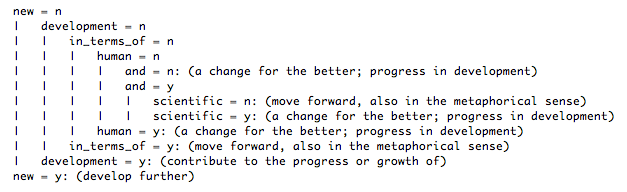
\includegraphics[scale=0.75]{./advance}
  \caption{Tree for \textit{advance}}
  \label{fig:treeAdvance}
\end{figure}

%\subsection{Training Data Set}
%\label{trainingdataset}
%\paragraph{}
%We make use of the widely used \textsc{SemCor}[to be cited] for our training data set. Specifically we use the tagged Brown Corpus files, with all content words tagged, of \textsc{SemCor}1.7.1. From this training data set, we retrieved a total of 20450 lemmas. Each lemma has a collection of sentences that that contain the lemma itself. Each sentence is an instance of the \textit{environment} that determines the word sense of that lemma. To capture these information, each lemma has an ARFF file, with all the words in the sentences as the \textit{attributes}, and the sentences themselves as the \textit{data instances}. In addition, we added an additional attribute to each ARFF file, \textit{WordNetSenseKey}, which captures the corresponding word sense for each data instance.

%\paragraph{}
%To generate the ARFF files for a target word, we first extract all sentences that contain the target word. We retain the WordNet sense key information found in the \textsc{SemCor} tagged files, and also the words' occurrence form. What follows is to specify each non-target word as an \textit{attribute} of its ARFF file, and each \textit{data instance} would represent each sentence. Each of these attributes would only have a true or false value, representing whether it exists in a particular sentence. Last, we add an additional attribute, \textit{WordNetSenseKey}, which captures the list of all sense keys available for that target word in the tagged files. \\
%\begin{figure}[htbp]
%@relation act \\ \\
%@attribute It \{\textit{n,y}\} \\
%@attribute recommended \{\textit{n,y}\} \\
%$\vdots$ \\
%@attribute WordNetSenseKey \{\textit{key 1},\textit{key 2}, $\ldots$ , \textit{key n}\} \\ \\
%@data \\
%\textit{y,y,n, $\ldots$ ,key 5} \\
%$\vdots$
%\caption{Sample ARFF file, \textit{act.arff}}
%\label{fig:sampleArff}
%\end{figure}
%\begin{figure}[htbp]
%  \centering
%  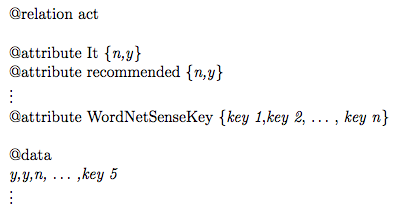
\includegraphics[scale=0.7]{./arff}
%  \caption{Sample ARFF file, \textit{act.arff}}
%  \label{arff}
%\end{figure}

%\paragraph{}
%On the side note, we saved the actual WordNet sense key in a separate location in order to keep the ARFF file free from attribute values that contains too many characters. For example, for \textit{act.arff}, the last attribute would only have values $1,2,\ldots,n$. The actual sense keys are saved in \textit{act.senselist}, which has a corresponding list of sense keys.

\section{Predicting Word Sense}
%\paragraph{}
%To predict the word sense of a target word, our system makes use of the sentence, which a target word occurred in, as the ``environment'', in other words context, of the word itself. The existence of certain words would contribute to an ambiguous word's sense in that sentence itself. For instance, consider the word \textit{bank}. It is logical, that if a sentence with the word \textit{bank} also contains the word \textit{interest} or \textit{financial}, we know that \textit{bank} here is \textit{likely} to refer to the place where we would have a savings account etc. In other case where the sentence contains \textit{river}, we can probably go fishing at this \textit{bank}.
\paragraph{}
Prediction of a target word begins with capturing the entire sentence the target word resides in. This is the \textit{environment} we mentioned in our intuition. 
Consider a sentence with only one ambiguous word to be disambiguated.%% Aobo: no connection between these two sentences 
 So we use the rest of the sentence to predict the word sense of that target word. Consider a set of all English words, $\varepsilon = \{$all English words\}. Ignoring the order of words and repeated usage of the same word in the same sentence, an English sentence can be denoted as a set of English words, as such: $S_{i} = \{a_{1}, a_{2}, \ldots, a_{k}\},~S\subseteq \varepsilon$. Therefore, suppose we perform WSD on $a_{j}$, we consider the set $S - \{a_{j}\}$ as its \textit{environment} that determines its word sense.

%\paragraph{}
%The next step is to create a data instance, and test it against an existing ARFF file. We first lemmatize $T$, then we check whether an ARFF file for the lemma $T_{lemma}$ exists. Suppose it exists. Then we generate a temporary ARFF file for $T_{lemma}$, such that its attributes are the same as the existing one in the training data set. Finally we use this temporary ARFF file to test against the training file, and hence outputs the prediction from our system.

\paragraph{}
In order to test for $a_{j}$, we check our training data set for existing data about $a_{j}$. Using the set $S_{i} - \{a_{j}\}$, we generate a single data instance to test against our training data. From there we utilize the Weka's Java packages to predict the word sense of $a_{j}$.

\paragraph{}
We test our system for the \textsc{SensEval} and \textsc{SemEval} all-words tasks. We pre-processed the test corpus such that we were able to test sentence by sentence. For all the sentences, we removed all quotations and punctuations, retaining only the English words as we only consider the actual words for word sense predictions.

\paragraph{}
In the following sections, we describe our implementation of the system in iterations. We will also provide the test results at each respective stage. We conducted our experiments using \textsc{SemCor1.7.1} as the training corpus for all the test corpus we were testing against. Our \textit{Baseline} is the WordNet-Sense-One, which assigns the most frequently tagged sense as the answer. The results of the WSD accuracies are shown in Table \ref{tab:resultsSum}.
%%From Chen Tao:  In Table3.3 you use WNs1 as the abbreviation of WordNet-Sense-One, it will be better if you explicitly write the abbreviation here.

\section{Iteration 1 (DT v0.1)}
\label{it:1}
\paragraph{}
Suppose we are performing WSD for every word in a sentence, a single-instance test file is generated for every testable word in the sentence. Then for each test file we run the prediction process to get the word sense. Consider the following example: \\

\begin{figure}[h]
\center
Before: the \textbf{quick} \textbf{brown} fox jumps \textbf{over} the lazy \textbf{dog} \\
\hspace{18 mm}After: the \textbf{quick}(\textbf{1}) \textbf{brown}(\textbf{1}) fox jumps \textbf{over}(\textbf{2}) the lazy \textbf{dog}(\textbf{1})
\caption{Output from iteration DT v0.1}
\end{figure}

\paragraph{}
In this example, the bold words are ambiguous, and we run them through the prediction process. The numbers in brackets are the results of the prediction process, and each of them refers to their corresponding word sense. The actual sense keys are stored in a different location to make the output cleaner.

\paragraph{}
In this iteration, the only feature we used is the occurrence of the neighboring words of a testable word, the \textit{environment} as we defined. As we were experimenting on this iteration, we quickly noticed that the speed of the prediction process was very slow. On average, the time taken to perform WSD on a sentence can easily be \textbf{10 to 40 seconds}. We picked a few random sentences from the test corpus to make comparison with the IMS system by \cite{itmakessense}, and the IMS performs at least 70\% faster than our system. Also, we compared our model size with IMS's, and our system's model size was twice as large (refer to Table \ref{tab:modelSize}). We address this two issues in Iteration 2.

\begin{table}[h]
	\center
	\begin{tabular}{| c | c |}
		\hline
		& Model Size \\
		\hline
		IMS & $\approx$ 275MB \\
		\hline
		DT v0.1 & $\approx$ 545MB \\
		\hline
	\end{tabular}
	\caption{Model size comparison}
	\label{tab:modelSize}
\end{table}

%\paragraph{}
%In this implementation, we make predictions using the model files generated using the J48 classifier. However, when we compared our model files with the model files of the IMS system, we found it to be 2 times as large (refer to Table \ref{tab:modelSize}). We concluded that in our model files, there are too much redundant information that is not used during the prediction process.

%\paragraph{}
%In our training data, information are captured in the form ARFF files. The attributes in these files are all the non-target words of the sentences. We captured these words as they are, and we did not perform lemmatization on them.

\section{Iteration 2 (DT v0.2)}
\label{it:2}
\paragraph{}
We found that in our model files, there are a lot of information that we can omit. More specifically, we only require the actual \textit{tree} itself for the prediction process, like the one illustrated in Figure \ref{fig:treeAdvance}. Hence we extracted only these trees, and further compacted the output such that each tree is now represented in a single line, as illustrated here:
\begin{center}
\textbf{advance$>$}new=n!$|$development=n!$||$in-terms-of=n!$|||$human=n!$||||$and=n:1(4/1)!$||||$and=y!$\ldots$
\end{center}

\paragraph{}
With this we compacted all trees into a single file, having the size of approximately \textbf{1 MB}. At this point, we were able to keep our model size very small, and to fulfill one of our goals: Size of Model.

\paragraph{}
Since the format of the model files was modified, the prediction procedures were also modified. In the modified procedures we dropped the usage of Weka to process the test instance. So we also did not need to generate a temporary test instance file to test against the existing file in our system. Instead, we used the trees extracted and treated each node as a test condition. So prediction means testing against nodes of the tree, eventually leading to a leaf node that provides a word sense.

\paragraph{}
We evaluated this iteration of our system to first make sure that the WSD accuracy remain the same, and also to determine the time taken. In the previous version, the prediction process for just one sentence can easily take 10-40 seconds, depending on length of the sentence. In the new procedure, all the trees are captured within a single file and we load the entire file into memory during the prediction process, in the form of a hash. With that, we were able to process all sentences from the three test corpus we tested against in approximately 2 minutes, averaging at about \textbf{0.10 seconds} per sentence. Compared to the previous iteration, we were able to reduce the time taken by at least \textbf{98\%}. With that we had also fulfilled the other goal: Speed.

\begin{table}[h]
	\center
	\begin{tabular}{| l | c | c |}
		\hline
		& Before DT v0.2 & DT v0.2\\
		\hline
		Model Size (MB) & 545 & \textbf{\large{1}} \\
		\hline
		Time Taken (secs per sentence) & 10 to 40 & \textbf{\large{0.10}} \\
		\hline
	\end{tabular}
	\caption{Comparison of model size and time taken}
	\label{tab:spaceandtime}
\end{table}

\section{Iteration 3 (DT v0.3)}
\label{it:3}
\paragraph{}
In the previous iteration, we did not lemmatize the attributes in our training data files. We speculated that if we lemmatize the attributes, we should be able to get better results compared to the previous implementation. By lemmatizing the attributes, we remove redundant attributes. For example, ``ate'' and ``eat'', where ``ate'' is considered redundant, since our system does not consider the tense of words. By doing so we also remove redundant nodes in the trees generated from the decision tree learner. For that the size of the new model trained from a new version of training data set was further reduced by \textbf{2\%}, from 1,052,703 to 1,032,414 bytes. Zooming in to each lemma's tree, we have reduction of tree sizes of up to \textbf{22\%}.

\begin{table}
	\begin{tabular}[h]{| l | c | c | c |}
		\hline
		& \textsc{SensEval-2} (\%) & \textsc{SensEval-3} (\%) & \textsc{SemEval-2007} Coarse-Grained (\%) \\
		\hline
		%Baseline & 62.4 & 58.9 & 73.0 \\
		Baseline (WNs1) & 55.9 & 48.8 & 64.3 \\
		\hline
		%DT v0.1 & 51.3 & 48.8 & \textbf{78.9} \\
		DT v0.1 & 48.5 & 45.5 & 57.8 \\
		\hline
		%DT v0.2 & 55.1 & 49.4 & 79.3 \\
		DT v0.2 & 48.5 & 45.5 & 57.8 \\
		%\hline
		%DT v0.1 + confidence & 54.8 & 50.1 & 79.3 \\
		\hline
		DT v0.3 & 49.2 & 46.2 & 58.3 \\
		\hline
		IMS & 68.2 & 67.6 & 82.6 \\
		\hline
	\end{tabular}
	\caption{WSD accuracies on \textsc{SensEval} and \textsc{SemEval} all-words tasks}
	\label{tab:resultsSum}
\end{table}

\paragraph{}
In this iteration we also added the \textit{confidence} feature, whereby if the confidence in the prediction is too low%%bellow a threshold 0.5?? give the number 
, we will switch to using the first sense of WordNet, that is, the sense with most frequency count. The value of confidence ranges from 0 to 1. As illustrated in Figure \ref{fig:outputDTv0.2}, the confidence values are now reflected alongside the prediction.

\begin{figure}[h]
\begin{flushleft}
\vspace{5 mm}
\hspace{10 mm}Before: the \textbf{quick} \textbf{brown} fox jumps \textbf{over} the lazy \textbf{dog} \\
\hspace{10 mm}After: the \textbf{quick}(\textbf{1:0.71}) \textbf{brown}(\textbf{1:0.97}) fox jumps \textbf{over}(\textbf{2:0.92}) the lazy \textbf{dog}(\textbf{1:0.98})
\end{flushleft}
\caption{Output from iteration DT v0.2}
\label{fig:outputDTv0.2}
\end{figure}

\paragraph{}
We evaluated our system with this new iteration and we attained improvements for all the corpus we tested against (refer to Table \ref{tab:resultsSum}). With this we demonstrated that even with a reduction of model size, we were able to attain an improvement in WSD accuracy.

\paragraph{}
For the time taken to perform WSD, we evaluated our system against the IMS system. Our system's model size is approximately 1MB, whereas IMS's is about 275MB. During the WSD process, both systems would need to load their models into memory. Clearly, loading IMS's model would take a longer time. In order for the comparison to be more fair, the number of test sentences have to be large enough so that the loading time would be less significant in the total amount of time taken. For that we use all the sentences we parsed from the test corpus, \textsc{SensEval-2}, \textsc{SensEval-3} and \textsc{SemEval}, to form a single test file of \textbf{789} sentences.

\begin{table}[h]
\center
\begin{tabular}{| c | c | c |}
\hline
& IMS & DT v0.3 \\
%& DT v0.3 Modified \\
\hline
For 789 sentences & 50.322 secs & 81.148 secs \\
%& \textbf{46.074 secs} \\
\hline
Time Taken per sentence & 0.0637 secs & 0.103 secs \\
%& \textbf{0.0584 secs} \\
\hline
\end{tabular}
\caption{Speed Test Experiment 1}
\label{tab:speedTest}
\end{table}

\paragraph{}
Our system loads the model into memory every time it performs WSD on a new sentence. For IMS, its model files are loaded only once to perform WSD on all 789 sentences. The time taken for this speed test is summarized into Table \ref{tab:speedTest}. Clearly, when performing WSD on large amount of text, IMS performs about \textbf{38\%} faster when compared with DT v0.3.
\paragraph{}
However this is not the intended nature for our system. Our system is meant to only perform WSD on a single sentence. In order to illustrate how our system actually performs, we need to perform a second speed test.

\begin{table}[h]
\center
\begin{tabular}{| c | c | c |}
\hline
& IMS & DT v0.3 \\
\hline
For 62 sentences & 17.636 secs & \textbf{\large{7.611 secs}} \\
\hline
Time Taken per sentence & 0.284 secs & \textbf{\large{0.123 secs}} \\
\hline
\end{tabular}
\caption{Speed Test Experiment 2}
\label{tab:speedTest2}
\end{table}

\paragraph{}
In this second speed test, we picked \textbf{62} random sentences from the test corpus. We ran these sentences through both system for \textbf{10} rounds each, and computed the average score for each round. For this speed test, we used the original DT v0.3 to compare against IMS. Making reference to the figures in bold in Table \ref{tab:speedTest2}, our system is faster in this speed test, when the setting is only to test for small amount of text. The speed performance of our system fulfills one of our goals: Speed. 
%\chapter{Evaluation}
\label{evaluation}
\paragraph{}
In our evaluation, we tested against \textsc{SensEval} all-words and \textsc{SemEval2007} coarse grained all-words tasks. We used WordNet 1.7.1 as our sense inventory.

\section{Pre-Processing}
\paragraph{}
Our method makes use of an entire sentence to predict the word sense of each word. The test files of \textsc{SensEval} and \textsc{SemEval} are in the XML format, so before can run through the all-words test files through our system, we had to pre-process the test files such that we were able to test sentence by sentence. For all the sentences, we removed all quotations and punctuations, retaining only the English words as we only consider the actual words for word sense predictions.

\section{Experiment}
\paragraph{}
We conducted our experiments such that we were using \textsc{SemCor1.7.1} as the training corpus for all the test corpus we were testing against. We pre-processed the \textsc{SensEval} and \textsc{SemEval} test corpus into sentences, then we ran the prediction process for all testable words in the test corpus. The results of the WSD accuracies are as shown in Table \ref{tab:resultsSum}.
%%Aobo: again, you have a table without any descriptions. Give discussions on the table

\begin{table}
	\begin{tabular}[c]{| l | c | c | c |}
		\hline
		& \textsc{SensEval-2} (\%) & \textsc{SensEval-3} (\%) & \textsc{SemEval-2007} Coarse-Grained (\%) \\
		\hline
		Baseline & 62.4 & 58.9 & 73.0 \\
		\hline
		DT v0.1 & 51.3 & 48.8 & 78.9 \\
		\hline
		DT v0.2 & 55.1 & 49.4 & 79.3 \\
		%\hline
		%DT v0.1 + confidence & 54.8 & 50.1 & 79.3 \\
		\hline
		DT v0.3 & & & \\
		\hline
		IMS & 68.2 & 67.6 & 82.6 \\
		\hline
	\end{tabular}
	\caption{WSD accuracies on \textsc{SensEval} and \textsc{SemEval} all-words tasks}
	\label{tab:resultsSum}
\end{table}

\section{Problems Faced}
\paragraph{}
Our post-experiment analysis helped us identified some problems that might had contributed to the results. Also, in this section, we review on whether our performance indicators were satisfied.

\subsection{Amount of Corpus Overlap}
\begin{table}[h]
	\center
	\begin{tabular}{| c | c | c |}
		\hline
		\textsc{SensEval-2} (\%) & \textsc{SensEval-3} (\%) & \textsc{SemEval-2007} Coarse-Grained (\%) \\
		\hline
		67.6 & 65.6 & 84.7 \\
		\hline
	\end{tabular}
	\caption{Corpus overlap with \textsc{SemCor1.7.1} (with respective test corpus)}
	\label{tab:overlapPercentage}
\end{table}
\paragraph{}
In the \textsc{SensEval} and \textsc{SemEval} test files, there exists some lemmas that are not found in our training data set which is generated from \textsc{SemCor}. Table \ref{tab:overlapPercentage} summarizes the percentage of overlap with \textsc{SemCor1.7.1}, with respect to each test corpus.

\paragraph{}
As you can see, the amount of overlap is consistent with the results shown in Table \ref{tab:resultsSum}. When the amount of overlap is lower, 67.6\% and 65.6\% for \textsc{SensEval-2} and \textsc{SensEval-3} in Table \ref{tab:overlapPercentage}, the performance is also lower, at 55.1\% and 49.4\% for \textsc{SensEval-2} and \textsc{SensEval-3} in Table \ref{tab:resultsSum}. When the amount of overlap is higher, at 84.7\% for \textsc{SemEval}, the performance is also higher, at 79.3\%. This shows that the amount of overlap in the corpus also affects the accuracy in WSD, the higher the amount of overlap, the more accurate the performance.

\subsection{Space \& Time Taken}
\paragraph{}
As mentioned earlier, our performance indicators are Accuracy, Speed and Size of Model.
\paragraph{}
A quick check on the size of our model files before Iteration 3 in Section \ref{it:3}, we found it to be twice as large when compared to IMS's model files (refer to Table \ref{tab:modelSize}). We concluded that in our model files, there are too much redundant information that is not necessary during the prediction process. In fact, during the prediction process, we only require the actual decision tree itself in order to predict word senses. Hence we extracted only the tree structure necessary for word sense prediction.

\paragraph{}
Using only the tree to predict word senses, and after further compression, we were able to reduce the model size to approximately \textbf{1 MB}.

\paragraph{}
Before we switch to the tree-only model files, the time taken to process each sentence easily took about \textbf{10-40 seconds}. The main reason for this is the length of the sentence, and the number of test-able words in that sentence. The longer the sentence, the longer it takes to process the entire sentence. After switching over to using the tree-only model files, the time taken was reduced significantly. We were able to process each sentence at an average of \textbf{0.15 seconds}  %combined together with chapter 3
\chapter{Conclusion}
\label{conclusion}
\paragraph{}
In this paper we focused on the need of a Word Sense Disambiguation (WSD) system that is directed at keeping the model size and time taken small. We found that even though there is much study made on WSD, few focused on introducing \textit{portability} into the system. For such a system, we intended to keep the size of model to minimal, while attempting to retain a reasonable level of accuracy. We opted to reduce the amount of pre-processing, like POS tagging, prior to the prediction of word senses. We believed that by doing so we incur additional supporting data, which increases the size of model. Also, we wanted to build a system that is speedy and responsive, so as to enhance users' experience. We wish to implement such a system so that we can perform real-time WSD on platforms like web browsers, or even mobile devices. On these platforms, we expect users to only perform WSD on small amount of text, like a sentence. For the project we identified three goals, namely: Accuracy, Speed and Size of Model.
%%Aobo: here you mention Acc but miss in Chapter 3
\paragraph{}
%% Aobo : if this is the motivation, do some comparision
We used Decision Trees in our system. It is simple to interpret and understand. It requires little data preparations, and able to have value even with little hard data. It is able to process large amount of data in a short time. We use the Weka implementation of the J48 decision tree learner to generate the model files to help us predict word senses.

\paragraph{}
In our system, we used \textsc{SemCor1.7.1} as our training corpus. Following our intuition on how the system would work, we extracted the training data sentence by sentence, so that each sentence serves as the \textit{environment} for each ambiguous word. For evaluation we tested our system against the all-words tasks of \textsc{SensEval-2}, \textsc{SensEval-3} and \textsc{SemEval}.

\paragraph{}
We acknowledge that our system produces low WSD accuracies. It seems a better choice to use the Baseline, which is fast, only requires a sense inventory file of about 7MB and has a higher accuracy. However there is still plenty of room of improvement for our system. As of now, the \textit{only} information that our system use is the occurrences of neighboring words. It does not have any other information, such as parts-of-speech, in the training and testing sentences. There are many other surface lexical features that can applied into our system. For example, we can add the \textit{bigrams} feature as described by \cite{pederson}. Otherwise, we can adopt collocations, which is also featured in IMS's system. Considering the potential for growth, our system is still better than the Baseline.
%%Aobo: do you have any experiemnts on these new features?

\begin{table}[h]
	\center
	\begin{tabular}{| c | c | c |}
		\hline
		\textsc{SensEval-2} (\%) & \textsc{SensEval-3} (\%) & \textsc{SemEval-2007} Coarse-Grained (\%) \\
		\hline
		67.6 & 65.6 & 84.7 \\
		\hline
	\end{tabular}
	\caption{Corpus overlap with \textsc{SemCor1.7.1} (with respective test corpus)}
	\label{tab:overlapPercentage}
\end{table}

\paragraph{}
We conducted additional post-experiment analysis and it helped us identified that the amount of overlap of the training and test corpus affected the WSD accuracies. Comparing Table \ref{tab:resultsSum} and \ref{tab:overlapPercentage}, we can see that the percentages in overlap are consistent with the performances in various test corpus. In other words, the higher the overlap, the higher the performance.

\paragraph{}
Though our analysis on the amount of corpus overlap showed that it played a part in the performance, it also showed the weakness of our system's inability to process \textit{unknown} words to the system. An immediate course of action from this point might be to increase the amount of training data, rather than only using \textsc{SemCor1.7.1}. Since our system captures training instances by sentences, we can \textit{learn} from WordNet itself, as WordNet do provide sample sentences for most of the words in its inventory. The advantage in this move is that it would expose the system to more words and senses. However, it also increases the system's dependency on a lexical database. Increasing the size of training corpus would directly increase the size of the model and conflict with one of our goals | to reduce the size of model in order to make the system portable. Furthermore, in \cite{yarowsky}, the authors reported that doubling the corpus would only reduce errors by 3 to 4\%. Therefore, in the longer term, we wish to introduce some \textit{unsupervised} characteristics to the system, so that it is less dependent on back-end resources.

\paragraph{}
Through the various iterations of our system's implementation, we demonstrated that we reduced the time taken and size of model needed to predict word senses. Prior to switching our system to use a modified model, the prediction process easily took 10-40 seconds to process a single sentence, and the size of model, at more than 545MB, was very large. We changed how we store our model and how we perform the WSD procedure, we reduced the time taken to an average of 0.10 seconds per sentence, and the size of model to only 1 MB.

\paragraph{}
We claimed that our system is able to perform speedily and responsively. To justify that we conducted 2 speed tests. The conclusion drawn from these speed test is our system performed at least twice as fast compared to the IMS system when performing WSD on a single sentence. This satisfies our intention to implement such a system into real-time applications like web browsers and mobile devices. We make reference to previous work done on DiCE Translator\footnote{https://addons.mozilla.org/en-US/firefox/addon/dice-translator/} prior to this system. As a Firefox plugin, DiCE's purpose is to provide bilingual translations for text on web pages to encourage language learning across a second language. Despite after extracting dictionary content from Wiktionary\footnote{http://www.wiktionary.org/}, DiCE lacks the ability to translate accurately according to the context. Integrating our system into DiCE, we plan for DiCE to be able to translate more relevantly, while still maintaining the overall responsiveness in using the tool.

%\paragraph{}
%As for WSD accuracy itself, our system was able to attain 79.3\% accuracy in the \textsc{SemEval2007} task. Our performance in this task came close with IMS's performance in the same task. From this we had shown that using Decision Trees, with minimal pre-processing, is a feasible method for word sense prediction.

\paragraph{}
There are many systems that attain high accuracies in WSD tasks. However, few the take size of model and time taken into consideration. We demonstrated that our system is able to keep both the model size and time taken to the minimal. To conclude, we had successfully created a system that is light-weight and speedy.
%%From Chen Tao:The second sentence "However, few the take..." may revise into "However, few of them take... into consideration." 
%\chapter{Future Work}
\label{futurework}
\paragraph{}
The immediate extension to this system would probably the bigram feature described by \cite{pederson}. Of course, we can adopt other forms of surface lexical features, like collocations, which is also featured in IMS's system. At this point, our system is a rather ``blind'' system, for it does not have any information about part-of-speech in the training and testing sentences. Hence the possible course of action would be include POS tagging features into the system, so that we would be able to attain higher accuracy.

\paragraph{}
Our analysis on the amount of overlap in the corpus, though it showed that it played a part in the performance, it also showed the weakness of the system's inability to process \textit{unknown} words to the system. An immediate course of action from this point would probably to expand the training data set, other than only using \textsc{SemCor}. Since our system captures training instances by sentences, we could possibly \textit{learn} from WordNet itself, as WordNet do provide sample sentences for most of the words in its inventory. The advantage in this move is that it would probably increase the system's WSD accuracies. However, it also increases the system's dependency on a lexical database. Increasing the size of training corpus would directly increase the size of the model and conflict with one of our goals | to reduce the size of model in order to make the system portable. Therefore, in the longer term, we wish to introduce some \textit{unsupervised} characteristics to the system, such that it would be less dependent on any back-end resources.
 %combined together with chapter 5


\bibliographystyle{socreport}
\bibliography{bibsource}

\appendix

\end{document}
